%% Mẫu luận án tiến sĩ (thạc sĩ) theo style vietkey.luanan.1.2.cls - Version 1.2
%% (c) Dang Minh Tuan, Vietkey Group.
%% Tel: +84-98-868-6636, Email: tuanvietkey@gmail.com.
%%
%% History:
%% - version 1.2 (2017/08/11)
%% - Created on 2016/08/16.

\documentclass[fontsize=13pt,oneside,a4paper,openany]{vietkey.luanan.1.2}

%tham số firstinits=true để viết tắt, defernumbers để số thứ tự liền mạch.
\usepackage[backend=bibtex,
            bibstyle=luanan,
            sorting=nyvt,
            block=none,
            %defernumbers=true,
            babel=other]{biblatex}
\usepackage{titling}
\usepackage{setspace}
\usepackage{fancyvrb}
\usepackage{dirtytalk}
\usepackage{listing}

\addbibresource{../bibdmt.bib}                 %%% dữ liệu về tài liệu tham khảo.
\begin{document}

\begin{titlingpage}
\begin{singlespace}
% \calccentering{\unitlength}
% \begin{adjustwidth*}{\unitlength}{-\unitlength}

\begin{center}
{\Large \textsc{Vietnam National University \\Ho Chi Minh city University of Techonology}\\
\vspace{3mm}
Faculty of Computer Science and Engineering
}\\
\vspace{10mm}
% \vspace*{13mm}
\includegraphics[width=0.3\textwidth]{images/logo.png}\\
\vspace{1cm}
\rule[0.5ex]{\linewidth}{2pt}\vspace*{-\baselineskip}\vspace*{3.2pt}
\rule[0.5ex]{\linewidth}{1pt}\\[\baselineskip]
{\huge \textcolor{blue}{Windows Memory Forensics}}\\[4mm]
{\Large \textit{\textcolor{blue}{Finding hidden processes in a running machine}}}\\
\rule[0.5ex]{\linewidth}{1pt}\vspace*{-\baselineskip}\vspace{3.2pt}
\rule[0.5ex]{\linewidth}{2pt}\\
\vspace{6.5mm}
{\large By}\\
\vspace{6.5mm}
{\Large\textsc{NGUYEN Anh Khoa - 1611617}}\\
{\Large\textsc{\textbf{Major}: Computer Science}}\\
\vspace{12mm}

\begin{minipage}{12cm}
A dissertation submitted to the University of Technology, VNU-HCM in accordance with the requirements of the DEGREE OF ENGINEER in Computer Science.
\end{minipage}\\

\vspace{6mm}
\begin{center}
\begin{tabular}{ r l }
\textbf{Instructors}:& \Large \textsc{Dr. NGUYEN An Khuong}\\
& \Large \textsc{Mr. NGUYEN Le Thanh}\\
& \Large \textsc{Mr. NGUYEN Quoc Bao}\\
\textbf{Opponent}:& \Large \textsc{Dr. TRAN Tuan Anh}\\
\end{tabular}
\end{center}
\vspace{7mm}
{\large Ho Chi Minh City, \textsc{July 2020}}
\end{center}
% \end{adjustwidth*}
\end{singlespace}
\end{titlingpage}
                          %%% có thể thay đổi

\VKnumRoman                                 %%% đánh số bằng chữ cái i, ii...

% \include{loicamdoan}                        %%% có thể thay đổi
% \include{loicamon}                          %%% có thể thay đổi

\clearpage
% \addcontentsline{toc}{section}{\abstractname}
\begin{abstract}

% Digital forensics is an action taken to extract raw data from computers and analyze that data to discover information or to learn about historical events that happened to the target machine. Computer forensics is more and more popular today where cyberattacks happen almost every day. When cyberattacks happen, we must stop the threat, but gathering information about the attack also has the same degree of importance. It is surprising how many information one can learn given only a snapshot of the memory, from running processes to hidden files and cryptographic keys. With high demands, people have come up with many techniques to analyze disk images, hard drives, and physical memory. No matter how great techniques we have for digital forensics, it is still worse than preventing an attack from happening. Even though Antivirus software, live reporting system and firewall mitigate some known attacks but with the new arising group of malware operate in stealth mode, like Cryptomining malware, or Rootkits remain a significant threat to organizations. In this paper, we would like to introduce a scanning system based on digital forensics to list running processes and to assist in the detection of malware.

Computers have become a tool that humans around the world use daily on for their study, work and entertain. With the capability to solve complex problems, it has become a necessity in our life. The widespread of computers also bring crime as hackers have been trying to damage the system or collect confidential information. Malware and attacks happen almost every day, threating our data. While anti-virus software and firewall cannot prevent new malware bringing new attack vectors, digital forensics act as a post-event investigation to collect and examine the attack. Memory forensics, a branch of digital forensics, dig into an infected machine finding hidden malware to analyze their behaviour. The job is done exclusively by experts and not available to the average user. If a regular user can know about the malware infecting his computer, we will be able to detect and prevent the possible spread of malware before the attack. Thus, we analyzed memory forensics techniques and proposed an implementation of a tool for finding hidden processes in a running machine, in the hope that this tool will run automatically and available to regular users as well.

\end{abstract}
\clearpage

\VKmucLuc                                   %%% mục lục

% \include{kyhieu}                            %%% có thể thay đổi

\VKdanhMucHinhVe                            %%% danh mục hình vẽ
\VKdanhMucBangBieu                          %%% danh mục bảng biểu
%\VKdanhMucDinhLy
%\VKdanhMucDinhNghia
\lstlistoflistings
\VKbatDaudanhSo                             %%% bắt đầu đánh số từ 1,2,3...

% \include{loinoidau}                         %%% có thể thay đổi
\chapter[Introduction]{Introduction}

In this chapter, we explain the definitions along with the current state of digital forensics and some contexts of today computer system and the current state we are in.

\section[Motivation]{Motivation}

Throughout the years of computer development, computers have become a standard method for humans around the world to study, work and entertain. Most activities of our daily lives involve computers. Individuals across the globe have created systems running on computers to assist them in doing common and complex tasks. However, this somehow influenced other people to commit harmful activities, these people often refer to as \textit{hacker}. Hackers have been creating software to cause damage and steal confidential or private information, these software are malware. Furthermore, lately along with the trend of cryptocurrency, while ordinary people commit their investment by using crypto mining machines, hackers, on the other hand, create sophisticated software (cryptojacking malware) that stealthily installed on a victim machine and mine cryptocurrency without the victim's acknowledgement.

Security researchers have been struggling to find ways to mitigate the gaining rate of attacks. However, it was never close to perfection. Security researchers uses file checksum and unique bytes sequences in file to create a file signature and combines a list of malware signature to a database, for example yararules \cite{yararules}. Relying on file signature database for filtering file often miss out new one, thus, it is highly vulnerable to the newer class of malware. To counterattack these new malware when an attack happens, digital forensics is performed. Digital forensics which as described by The Forensics Research Workshop I \cite{roadmap}:

\say{The use of scientifically derived and proven methods toward the preservation, collection, validation, identification, analysis, interpretation, documentation and presentation of digital evidence derived from digital sources for the purpose of facilitating or furthering the reconstruction of events found to be criminal, or helping to anticipate unauthorized actions shown to be disruptive to planned operations.}

Digital forensics includes many different aspects, however, the most intrigued part of digital forensics is memory forensics, which "provides unprecedented visibility into the runtime state of the system, such as which processes were running, open network connections, and recently executed commands" as stated in the book The Art of Memory Forensics \cite{ligh2014art}. Memory forensics provide a frame of the computer state, from which one can extract files and processes. Researchers often extract suspicious files from these memory samples, then reverse engineer it, if the file is a malware, they will create the file signature and add to the database. Digital forensics and memory forensics is very important to gain insight on the cyber attacks made by hackers. However, prevention is always better than fixing, and with the rise of the more steathy malware, the computer security industry is facing a major problem.

Malware are good pieces of software, but only before the disclosure. Therefore hackers creates malware hidden from the Task Manager and other process listing tools. From the early days of 1990s, they have been improving ways to hide malware. In 2017, a small report \cite{evolutionHidding} have revised on hiding techniques in malware over the years in the Windows OS. Most of these techniques is either preventable or mitigable. However, even in 2019, we can still observe incidences where malware hide itself so effectively. For example, Android malware that hid themselves on user mobile and was only found September 2019 after 5 months on the Google Play Store \cite{hiddenMalwareAndroid}, or the \textit{Titanium} backdoor\footnote{Programs that receives remote connections} on Windows 10 disclosed November 2019 \cite{titanium}, or the macOS malware, named \textit{unioncrypto}, that downloads and runs a hidden process in memory to mine cryptocurrency was only discovered December 2019 \cite{unioncrypto}. Researchers collected and analyzed these malware, but a normal user would not be able to do that. For a normal user, if the anti-virus software failed to flag the file as mallicious, his computer will be infected. To know whether a system is having a hidden malware running, one must send an investigator a memory extraction. Such process is complex, long and costly, a user must know how to extract the memory and hire an investigator to analyze. If there were a tool to do memory forensics live, while the system is running, and extract the hidden malware automatically, it would be easier for a normal user. Looking in live memory forensics, Shuaibur Rahman and Khan \cite{reviewLive} has a review of live forensics analysis techniques in 2015, and in the review there is one work that can extract running, finished, and cached processes \cite{comparativeLive}. However, the work is only restricted to the Linux OS and requires an experienced invetigator to do. Besides that, there are projects that implements memory forensics techniques but is limited to dump file analysis. We have researched for live memory analysis and have come up with a method for finding hidden processes.

Within the scope of the thesis, we will create a tool finding hidden processes aims at normal users. The tool could also submit the binary along with the process memory to the remote server. And with the market share of Windows over others OS is more than 75\% \cite{osMarketShare}, within the Windows OS, version 10 is now dominating with more than 60\% \cite{windowsShare}, this tool will focus on Windows 10 live memory analysis.

\section[Objectives]{Objectives}

In the scope of this thesis, we wish to:

\begin{itemize}
  \item Understand the basics concept of OS that supports memory forensics.
  \item Understand to some extend the internal of Windows operating system.
  \item Understand some techniques often used to do Windows memory forensics.
  \item Analyze some already existed tools doing memory forensics.
  \item Propose a method to find hidden running processes in a running Windows machine.
\end{itemize}

\section[Structure]{Structure}

% TODO


\chapter[Background]{Background}
\section[Operating System concepts]{Operating System concepts}

\subsection[Multiprogramming]{Multiprogramming}

Multiprogramming defines a computer where it can run serveral programs at the same time. To enable multiprogramming the OS must be capable of managing memory region for processes, scheduling running time for processes, and many more crucial tasks. We will briefly review the two aspect of multiprogramming.

The first aspect is scheduling. Cooperative multitasking, or so called non-preemptive multitasking, is a design for multiprogramming scheduling where it does not limit a process's runtime. A process will actively run until it stops/idles or waits for an I/O operation, whence the operating system will switch context to another process. In contrast with cooperative multitasking, preemptive multitasking limits the process's runtime and initiate a conext switch when the criteria is met. Both approach have been used in many operating systems but cooperative multitasking schema sometimes causes system to hang, thus in most modern operating system (Windows, MacOS, and most Linux distributions), preemptive multitasking schema is chosen.

\begin{figure}
  \centering
  \caption{Preemptive}
  \includegraphics[scale=0.8]{images/preemptive.png}
  \text{4 processes (A, B, C, D) running in a tiny time slot which appears simutaneously to a human}
\end{figure}

The second aspect is memory management. In the early days, memory management was so simple that it would contain the whole process consecutively in memory. However, doing this leads to external fragmentation\footnote{the memory is empty but not fit consecutively for a process}. Then people realize that it is not optimized to contain the whole process in memory because some part of it is unused at a specific point of time. For example, when we have a program with many functions, at one time we only run a few of them. To optimize this, people choose to load only the necessary parts in memory. After many years of optimizing, people have agreed upon splitting a process to equal parts called a \textit{page}. The OS split the physical memory to pages and load process to those pages. When a process needs more space or needs parts that are not on memory, the OS will find an empty/unused page to load in. If there is no empty page, one least use page will be swapped out to disk to make space. The OS tracks what pages a process is using and swap those pages in when the process needs.


So far, we have only discussed processes that have a limited amount of memory, but OS allows programs to have more space by using the paging technique describe above. A process can have a virtual space of addresses with which it can use. Every process running will have a certain amount of \textit{virtual} memory available. Assuming we have a process, that process will have 2GB of memory (from 0 to $2^{32}-1$) and at 0x40000000 is the start of \texttt{.text} section from that process point of view. However the page from \texttt{.code} to \texttt{.code + page\_size} is located in RAM at address 0x60000000 to 0x60000000 + \texttt{page\_size}. The OS has to translate the address from 0x40000000 to 0x60000000 when the process accesses any address in page size from 0x40000000. This is called \textit{address translation}. Although access to a memory section is more complex, by using virtual memory, a process can have more memory. If many processes use the same library, that library would be map over to a virtual section of that process.

\begin{figure}
\centering
\caption{External fragmentation}
\includegraphics[]{images/external_fragmentation.png}
\end{figure}

\begin{figure}
\centering
\caption{Splitting process}
\includegraphics[]{images/splitting_process.png}
\end{figure}

\begin{figure}
\centering
\caption{Splitting process}
\includegraphics[]{images/use_same_lib.png}
\text{Two processes use the same library (LIB B) and is visible in its own (virtual) address space}
\end{figure}

% TODO: Insert picture

% In modern OS design, people notice that a process not always needed everything to be in memory. Unused parts of a process can be transfered to secondary memory and bring it back to primary one on demand. OS does process spliting base on this theory, split one process into many parts and only load the part that is needed at that time. Spliting of the process can be done in many different ways, but spliting by a constant size is commonly used. This constant size is called a \textit{page}, and by most OS, this amount is 4KB by default. The physical memory is splitted by page also. Every process will have a private address space, called user-space, which one process can write/read and execute. This private address will contain all process's data, including code, data, and heap. All processes have a common shared address space which contains information available system wide, this space is called the kernel-space. Eventhough that all processes share the kernal-space they cannot access this address space due to OS prevention. These two spaces are virtual, the OS mechanism makes processes "think" that they owns a large memory region, while infact memory are splitted and located accross the primary or secondary memory. The picture below contains two processes running, while both of them are loaded the whole memory of the process is not neccessary to be in RAM. Both processes virtualy have a separated memory space, these memory region will be loaded to RAM on demand, and swapped out to disk when unused and the OS needs to load new pages in.

% The design of paging technique is very useful. A process can be splitted to many parts and only loads what is needed, furthurmore, processes that uses the same library can reuse the already loaded one and not neccessary to reload again. Because memory is scattered through the RAM and disks, and each process has a virtual memory space, the OS must keep track of Pages and Pages mapping. When a process access a memory address in the process space, the OS will translate to the physical address lies in RAM.

% \subsection[Multiprocessor]{Multiprocessor}


% \subsection[Threads]{Threads}


\section[Windows Internals]{Windows Internals}

To understand memory forensics on Windows, knowledge about Windows Internals is necessary, from memory model to some kernel design. In this section we will give the reader some technical details on Windows' design.

\subsection[Memory model]{Memory model}

We start by exploring the Windows memory model, and more importantly the Windows kernel memory model. Windows by default uses page size of 4KB, the virtual address space for each process is 2GB for the 32-bit version and 8TB for the 64-bit version. The system address space is 2GB for the 32-bit version and 248TB for the 64-bit version. For every processes, when run, can see both its own address space and the system space, but access to the system space is restricted. A typical 32-bit process can have a 2GB space for itself and a 2GB space of the system, makes a total virtual memory space 4GB. The system space, refer to as the kernel space, contains the OS kernel objects and the currently running drivers and kernel application. The kernel space uses \textit{pools} to manage objects allocation and deallocation. Windows has two types of pool, one that is \textit{pagable}, can swap out to disk, called \textit{paged pool} and the other \textit{non-paged pool}. The size of these two types of pool on Windows 10 can be reference through the Table~\ref{tab:poolsize} \cite{memorylimit}. Because many parts of the OS is not used often, Windows can swap those pages out to make more space. However, some information will always remained in the non-paged pools.

\begin{center}
\begin{table}[h]
\begin{tabular}{l p{5cm} p{5cm} }
Pool Type & Limit on 32-bit & Limit on 64-bit \\ \hline
Paged Pool & 384 GB or system commit limit, whichever is smaller & 384 GB or system commit limit, whichever is smaller \\
Non-paged Pool & 75\% of RAM or 2 GB, whichever is smaller. & RAM or 128 GB, whichever is smaller (address space is limited to 2 x RAM) \\
\end{tabular}
\caption{Pool size on Windows 10}
\label{tab:poolsize}
\end{table}
\end{center}

The memory pool is a bitmap\footnote{An array of bits}. Windows will return the pointer and size when asked for space in the pool (chunk). Windows keeps track of chunks in the pool. At first, there is only one chunk (the pool itself). When the user asks for space, Windows will split the chunk into two, one for the user and one left unused, Windows will keep spliting the unused space in pool and return to the user for any allocation requested. Upon deallocation, Windows will merge unused chunks into one. Consider the code in Listing~\ref{lst:basicpool} for a basic example of pool allocation.

% TODO: Picture

Each chunk will have a \texttt{POOL\_HEADER} field on top to denote the content of the chunk. \texttt{POOL\_HEADER} has a size field (\texttt{BlockSize}), a previous size field (\texttt{PreviousBlockSize}), and a tag (\texttt{POOL\_TAG}). Tag is a four-byte character that Windows and Driver writer use to denote the data stored in the chunk. In Table~\ref{tab:pooltag}, we listed some typical structure with its tag.
\lstinputlisting[language=C,caption={Basic Pool Algorithm},label={lst:basicpool},basicstyle=\linespread{0.8}]{code/basic_pool.cpp}

\begin{center}
\begin{table}[h]
\begin{tabular}{lll}
Structure     & Structure Name   & Pool Tag \\ \hline
Driver Object & \_DRIVER\_OBJECT & Driv     \\
File Object   & \_FILE\_OBJECT   & File     \\
Process       & \_EPROCESS       & Proc     \\
TCP endpoint  &                  & TcpE     \\
TCP listener  &                  & TcpL     \\
Thread        & \_ETHREAD        & Thre     \\
UDP endpoint  &                  & UdpA     \\
\end{tabular}
\caption{Some pool tag and corresponding structure}
\label{tab:pooltag}
\end{table}
\end{center}

\subsection[EPROCESS and ETHREAD]{EPROCESS and ETHREAD}

Windows has a special structure that contains a process information called \texttt{\_EPROCESS}. This structure is created every time when a new process spawns and located inside a non-paged pool with tag \textit{Proc}. If we have a reference to one \texttt{\_EPROCESS} we might follows \texttt{LIST\_ENTRY ActiveProcessLinks}, a doubly linked list pointer, to find other \texttt{\_EPROCESS} of different process Figure~\ref{fig:eprocesslink}. However because this structure can be accessed by a normal user by calling \texttt{PsLookupProcessByProcessId} one may edit the doubly linked list to remove itself from the list chain Figure~\ref{fig:dkom}.

\begin{lstlisting}[language=c,caption={LIST\_ENTRY},label={lst:listentry}]
typedef struct _LIST_ENTRY {
      struct _LIST_ENTRY *Flink;
      struct _LIST_ENTRY *Blink;
} LIST_ENTRY, *PLIST_ENTRY, PRLIST_ENTRY;
\end{lstlisting}

\begin{figure}[H]
\centering
\caption{EPROCESS Linking}
\label{fig:eprocesslink}
\includegraphics[]{images/eprocess_link.png}
\end{figure}

\begin{figure}[H]
\centering
\caption{EPROCESS linking modified}
\label{fig:dkom}
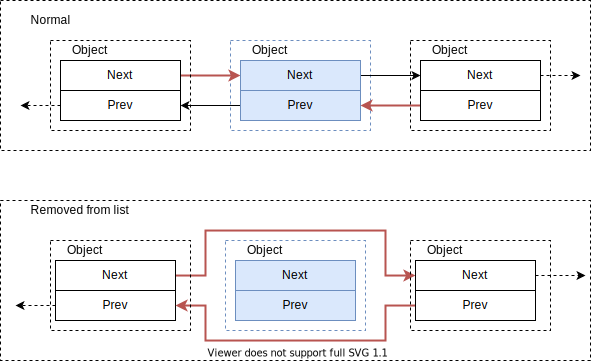
\includegraphics[]{images/dkom.png}
\end{figure}

A process in Windows is composed by threads, for example, a process loading a library will have the library run as a thread. Every thread will have a kernel object inside the non-paged pool to manage called \texttt{\_ETHREAD}. From an \texttt{\_ETHREAD} we can call \texttt{IoThreadToProcess} to get the parent \texttt{\_EPROCESS}, see Listing~\ref{lst:threadtoprocess}. \texttt{\_EPROCESS} has a doubly linked list of \texttt{\_ETHREAD} in \texttt{LIST\_ENTRY ThreadListHead} to list threads of a process.

\begin{lstlisting}[language=c,caption={IoThreadToProcess},label={lst:threadtoprocess}]
PEPROCESS IoThreadToProcess(
  PETHREAD Thread
);
\end{lstlisting}

\subsection[KDBG]{KDBG}

KDBG short for \texttt{Kernel Debugger Block} is one of the commonly used structure when analyzing a memory artifact of Windows. It was created to easy debugging process for developers when writing OS or kernel drivers. As this struture contains pointers to others structures. One pointer contained in KDBG is \texttt{PsActiveProcessHead} which is a pointer to an \texttt{\_EPROCESS}. As previously mentioned, we can walk the list of \texttt{\_EPROCESS} to enumerate all processes.

% TODO: Move this somewhere else

However from Windows 8, this structure is encoded and hinders us from analyzing windows memory. As quoted by the developers of Volatility \cite{kdbgEncoded},

\say{An encoded KDBG can have a hugely negative effect on your ability to perform memory forensics. This structure contains a lot of critical details about the system, including the pointers to the start of the lists of active processes and loaded kernel modules, the address of the PspCid handle table, the ranges for the paged and non-paged pools, etc. If all of these fields are encoded, your day becomes that much more difficult.}

While users of Volatility will suffer a bad day, Rekall's users do not as they use another method without knowledge of KDBG structure \cite{rekallOnKDBGEncoding}. However, KDBG is still an important Windows structure that provides kernel information.

\subsection[Windows dump file]{Windows dump file}

Windows provides a dump file to contains compressed memory data. This file is created by Windows when an error in kernel occur. Third party tools can dump the memory on running machine for example, DumpIt, FTK Imager. This file structure is not documented, however, it was written on Microsoft debug file, Schuster \cite{dmpfile} has written a guide to the file structure. Another dump file type is mini dump file which is documented by Joachim \cite{mdmpfile}. These dump files are commonly used to preserve the system memory state for analysis.

\subsection[Process injection]{Process Injection}
\label{sec:processinjection}

Process injection is a technique to inject a process to another running process. In 2019, Amit Klein and Itzik Kotler gave a talk at US Blackhat conference about the topic \cite{processinjection}. The research is done on Windows 10 x64, they tried to systemize the process injection techniques. Some techniques could still be used although Windows 10 has better security than previous Windows version. A process injected will be more stealthy since the system can only see the parent process. This method is often used by malware to make their process hidden from the system. However, for any process spawn, a thread is always created, so there is always an \texttt{\_ETHREAD} of the process.

\section[Digital Forensics and memory forensics techniques]{Digital Forensics and memory forensics techniques}

Digital forensics describes the process includes the collection and analyzation of evidence; information synthesization; and sometimes unknown binaries and files analysis. Digital forensics has become significant in the industry. People will turn into digital forensics companies when they notice or doubt one computer contains illegal files or malicious applications. Without digital forensics, we cannot traceback when an attack happens, and without prior learning of historical events, we can not build a more reliable system to detect and prevent future replicate attacks. We learn and build filters based on files signature\cite{yararules}. These signatures can be unknown from a Zero-day attack, and even a One-day attack can still harm the system. Digital forensics is gaining more and more important when the next generation of malware do not intend to break the system but to exploit the system computing power for profit or collect sensitive information. Most notably are Cryptocurrency Malware and Botnet; these types of malicious applications will run inside the system and uses little computations. Backdoors and trojans are another concern when they silently collect user's information, files and activities. We can only know of their existence when the attack had happened.

\subsection[Evidence gathering]{Evidence gathering}

Once we have identify the corrupted system, we must try to disconnect the machine from the internet. But if we disconnect the system from the internet, the malware will drop all connection and we will lose all traces. Hence, we must quickly dump the memory of the system and disconnect the machine from the internet. The memory dump will have these information:

\begin{itemize}
\item Currently running processes
\item Currently opening files (file descriptor)
\item Currently opening sockets
\end{itemize}

After acquisition of memory dump file, we use forensics tools and begin analysis. In the worst condition, where we must shutdown the system, we can try to collect the whole physical memory by using \textit{cold boot attack} \cite{coldboot}. This technique relies on memory data disolve slower on low temperature, enable us to shutdown and collect RAM data given physical access. Full RAM dump can easily be converted to dump file format to use with tools. After raw memory is gathered we will start analyzing. The two most notable tools for memory forensics are Google's Rekall platform, and the Open-source Volatility project. These two tools are used by most digital forensics teams.

Next we will describe some technique on memory forensics.

\subsection[KDBG scanning]{KDBG scanning}

Scanning KDBG will provides some small but important piece of information. As described in Windows Internal, KDBG has a pointer to PsActiveProcessHead, which is a pointer to the doubly linked list of \texttt{\_EPROCESS}. Volatility used KDBG scanning to characterize Windows version before Windows 8. From Windows 8 forward, this structure is encoded and made a hindrance to Volatility users.

\subsection[Pool tag scanning and quick scanning]{Pool tag scanning and quick scanning}

Pool tag scanning is a technique to find structure by scanning the pool first introduced by Schuster \cite{pooltagscan} in 2006. By ultilizing the pool layout with \texttt{POOL\_HEADER}'s \texttt{POOL\_TAG}, we can scan for tags that contains a certain structure. Physical memory is getting larger and scanning the whole address space is not suitable anymore. In 2016, Sylve, Marziale and Richard \cite{sylve2016pool} has improved the algorithm for 64-bit Windows by using a global kernel variable indicating the start of dynamic allocation and a pointer to allocation bitmap (\texttt{MiNonPagedPoolStartAligned} and \texttt{MiDynamicBitMapNonPagedPool}).


\chapter[Related works]{Related works}

\section[Volatility]{Volatility}

Volatility is an open-sourced forensic tools first developed by Aaron Walters and Petroni. It was first introduced in 2000 and by now Volatility has gain much popular in the digital forensics world. This work combines years of digital research into a convenient and versatile tool. The tool allows forensics investigators to analyze a memory dump file of Windows, macOS and Linux. It is designed by plugins of different version of OS, includings major, minor and build version. These plugins specify constatnt numbers, kernel structure definitions and others OS related information.



\input{chapters/rekall.tex}

\chapter[The proposed method]{The proposed method}

With the pool tag scanning described in Section \ref{sec:pooltagscanning}, we proposed a way to do it live. The steps are listed below for clarity:

\begin{enumerate}[label={Step \arabic*. },leftmargin=4\parindent]
  \item Run a controlled driver in kernel space
  \item Perform pool tag scanning
  \item Deserialize the bytes to get processes information
  \item Find potential hidden process and send to the server
\end{enumerate}

Our program should have two parts, part that runs inside the kernel space, \texttt{K}, and part that run in user space, \texttt{U}. We will perform pool tag scanning with \texttt{K} and for every successful findings, \texttt{K} will send the structure as bytes to \texttt{U}. From that \texttt{U} will try to extract information by deserialize the bytes to a defined structure.

\section[Run a controlled driver in kernel space]{Run a controlled edriver in kernel space}

Our tool needs a process, which is a kernel driver in this case, in order to gain access to the kernel space. The kernel driver can be loaded while booting the machine or by calling the undocumented Windows API -- \texttt{NtLoadDriver(PUNICODE RegistryPath)}. Both ways need a key that is registered at a specific path in the Windows registry, \texttt{\textbackslash registry\textbackslash machine\textbackslash SYSTEM\textbackslash CurrentControlSet\textbackslash Services}. The key must have three values:

\begin{itemize}
% \setlength\itemsep{-0.5em}
  \item \texttt{ImagePath}: the path of the driver to be loaded,
  \item \texttt{Start}: an enumeration specifing when to start the driver, manually or on boot,
  \item \texttt{Type}: an enumeration specifing the type of the driver.
\end{itemize}

To load the driver, the \texttt{Start} value should be \texttt{2} for automatically start and \texttt{3} for manually start. The \texttt{Type} value should be \texttt{1} for specifying the driver is in the type of kernel device. Once the driver is loaded and run, we have permission in the kernel space.

\section[Perform pool tag scanning]{Perform pool tag scanning}

Performing pool tag scanning for hidden processes requires a pointer to an address in the non-paged pool. Calling an allocation through \texttt{ExAllocatePoolWithTag(POOL\_TYPE PoolType, SIZE\_T NumberOfBytes, ULONG Tag)} will return a pointer to a chunk pool. By calling the function with \texttt{PoolType = NonPagedPool}, a pointer inside the non-paged pool will be returned. Using this pointer to scan the pool by the given algorithm, for each positive hit of \texttt{\_EPROCESS}, the driver will send the bytes of the structure to the user space process \texttt{U}. Continue scanning to get all the structures in the pool.

\section[Deserialize the bytes to get processes information]{Deserialize the bytes to get processes information}

After we have collected the raw bytes, they need to be deserialized to their correct structure based on Windows build. The Windows kernel structures change drastically over every builds \cite{windowsKernelCharacterization}. Thus, \texttt{\_EPROCESS} layout is not fixed across Windows builds. Kernel structure layout is important for driver developers, so Windows has a file to record these structures layout and distributed with every Windows builds. Those files are called PDB (program database). Windbg, the Microsoft debugger, and Visual Studio both use these file for debugging purposes. Microsoft hosts these files at \url{https://msdl.microsoft.com/download/symbols}. However, the download protocol is not HTTP. To download these files, one may need to use Windbg. Another option is to use \textit{pdb-downloader} by Rajkumar Rangaraj \cite{pdb-downloader}, the code is open-source and written in \textit{C\#}. The protocol can be understood through the code and re-implement to fit our needs.

The PDB files are now available, but, the file is not parsable now. The file format is not officially documented, Microsoft only gave the community an incomplete repository containing the PDB file information \cite{microsoft-pdb}. Fortunately, community over time have written many parsers, from these open-source parser, we can use to parse the PDB files and get \texttt{\_EPROCESS} structure definition. With the correct \texttt{\_EPROCESS} definition, the bytes will be deserialized in order to get information from the bytes. The information are the process identification number (process id), the process creation and exit time, and the file path. The information can be retrieved from these members of \texttt{\_EPROCESS}:

\begin{itemize}
% \setlength\itemsep{-0.5em}
  \item Process id: \texttt{PVOID UniqueProcessId}
  \item Process create time: \texttt{LARGE\_INTEGER CreateTime}
  \item Process exit time: \texttt{LARGE\_INTEGER ExitTime}
  \item File path: \texttt{UCHAR ImageFileName[16]}
\end{itemize}

\texttt{UniqueProcessId} is a pointer, in this case, the value must be dereferenced. The value is inside the kernel space, so the tool will request the driver to fetch the value. When all processes information is gathered, we have completed step 3.

\section[Find potential hidden process]{Find potential hidden process}

In step 4, with all the processes information collected from pool tag scanning, we will attempt to filter out normal processes. Normal processes are visible to the system and can be enumerated by traversing the \texttt{LIST\_ENTRY ActiveProcessLinks} of any process. To get an \texttt{\_EPROCESS}, we will call \texttt{PsLookupProcessByProcessId}, Listing~\ref{lst:pslook}, with the tool id. Filtering out process that is not on the list after traversing the \texttt{\_EPROCESS} will yield a list of potentially hidden processes.

\begin{lstlisting}[language=cpp,caption={PsLookupProcessByProcessId},label={lst:pslook}]
NTSTATUS PsLookupProcessByProcessId(
  HANDLE    ProcessId,
  PEPROCESS *Process
);
\end{lstlisting}

With the list of process id of malicious processes, we will dump the process memory and collect the binary file. For dumping a process from memory, we can use a tool created by Geoff McDonald \cite{processdump}. The binary file can be collected through the file path string extracted. Zipping all the dump files and binaries, we send the zip file to the server for further analysis. If the researchers find the file is a malware, they will write a script to stop and remove the malware from the computer and send back to the tool running for automatic removal. Ofcourse, there are time taken to analyze new sample, but we can notify the user through email that there is a malware running and ask the user to open the tool, enter the malware id, and receive automatic malware removal.

\chapter[Challenges and conclusion]{Challenges and conclusion}

\section[Challenges]{Challenges}

With the given proposed method above, we will name out some challenges the method might have and ways we can resolve those challenges.

Firstly, the proposed method is based on pool tag scanning, and thus, we should hit the same problem where pool tag scanning has. Pool tag scanning can scan deleted or freed process, where the pool chunks are merged but not overwritten. Pool tag scanning uses tag value, but any kernel driver can name these tag values, a hacker may write malware that allocates a false positive chunk with tag \textit{Proc}.

Secondly, the tool only scans for \texttt{\_EPROCESS} and may miss processes that were injected to another process as a thread. To resolve this, the tool could scan for \texttt{\_ETHREAD} and find the parent process \texttt{\_EPROCESS} using \texttt{IoThreadToProcess}. Then, from the given \texttt{\_EPROCESS}, loop through the \texttt{ThreadListHead} to find whether the thread is recorded in the process or not.

Thirdly, the hidden process activities are not monitored to send with the binary and the process memory dump. Process activities are significant to learn about file behaviour. It would be better if the result is attached with a log of process activities including file I/O and networking request/response.

Lastly, the algorithm using is not quick scanning. For a larger memory, it could result in long scanning time. Pool tag quick scanning would be a considerable improvement, but we will focus on implementing the standard algorithm and try to improve with pool tag quick scanning.

\section[Conclusion]{Conclusion}

In this proposal stage, we have researched thoroughly about memory forensics in Windows and have come up with a solution to perform live memory forensics for finding hidden processes running. Besides, our group has begun to start developing the prototype of the tool.

Within the next stage of the thesis, we will continue working on the implementation of the tool, perform testing and resolve the challenges mentioned above. We will also try to target lower Windows versions to test the usability of the tool.


% \include{ketluan}                           %%% có thể thay đổi
% \include{chdanhmuccongbo}                   %%% có thể thay đổi

\nocite{*}
\VKngatTrang                                %%% ngắt trang để chuyển sang tài liệu tham khảo
\VKtaiLieuThamKhao                          %%% tài liệu tham khảo
\VKdanhSoPhuLuc                             %%% bắt đầu đánh số cho phụ lục

% \include{phuluccaidat}                      %%% có thể thay đổi

\end{document}

